%Capitulo 7, presentación 21
\definecolor{DarkPurple}{RGB}{100,0,110}
\begin{frame}{Otros puntos estrechos}
	\begin{minipage}{0.35\textwidth}% adapt widths of minipages to your needs
		\quad\quad\quad 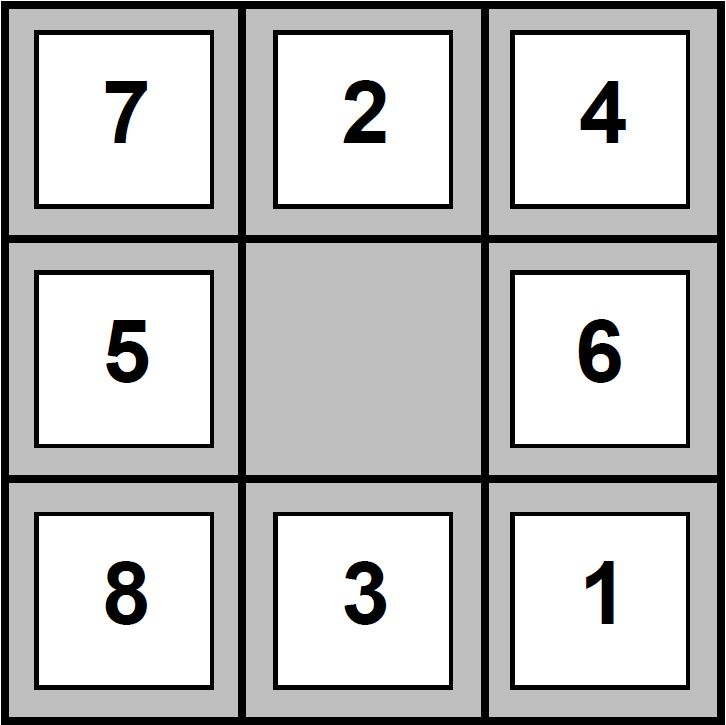
\includegraphics[scale=.3]{images/21_grid1.JPG} 
	\end{minipage}%
	\hfill%
	\begin{minipage}{0.65\textwidth}\raggedright
		{\footnotesize %scriptsize tiny
			\qquad Brisa en (1,2) y (2,1)
			\begin{itemize}
				\item[$­$]
				\begin{itemize}
					\item[$\Rightarrow$]sin condiciones seguras
				\end{itemize}
			\end{itemize}
			\qquad Asumiendo hoyos distribuidos uniformemente,
			\\
			\qquad (2,2) tiene un hoyo con prob 0.86, vs. 0.31
		}
	\end{minipage}
	\\
	\begin{minipage}{0.35\textwidth}% adapt widths of minipages to your needs
		\quad\quad\quad 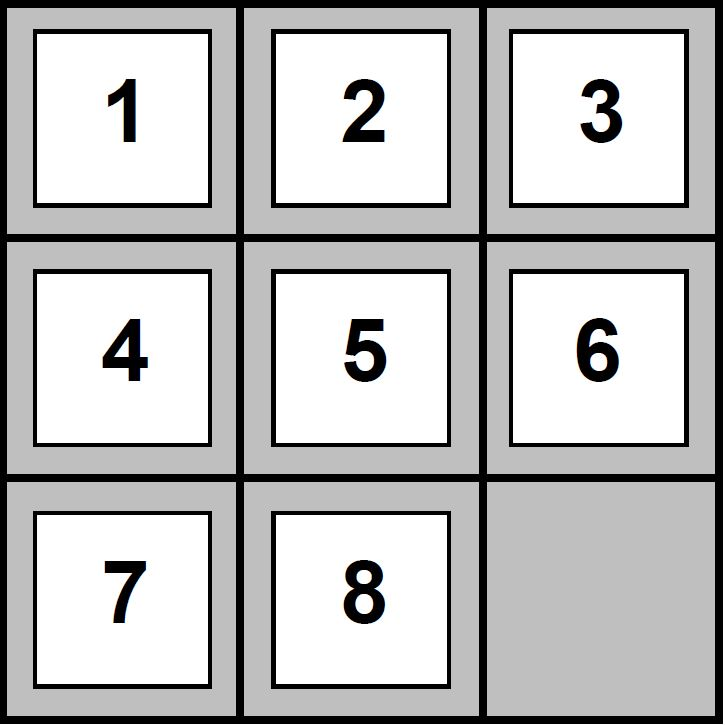
\includegraphics[scale=.3]{images/21_grid2.JPG} 
	\end{minipage}%
	\hfill%
	\begin{minipage}{0.65\textwidth}\raggedright
		{\footnotesize %scriptsize tiny
			\quad
			\\~\\
			Olor en (1,1)
			\begin{itemize}
				\item[$\Rightarrow$]no se puede mover
			\end{itemize}
			Se puede usar una estrategia de \textcolor{DarkPurple}{coerción}:
			\\
			\quad disparar en linea recta
			\\
			\quad wumpus estaba allí {$\Rightarrow$} muerto {$\Rightarrow$} a salvo
			\\
			\quad wumpus no estaba allí {$\Rightarrow$} a salvo
		}
	\end{minipage}
\end{frame}